\renewcommand{\thetable}{S\arabic{table}}
\setcounter{figure}{0}
\renewcommand{\thefigure}{S\arabic{figure}}

\section{Supplementary Materials}

\begin{sansmath}
\py{pytex_fig('scripts/vc_violin_bootstrap.py',
        conf='article/temp.conf',
        label='mscv',
        caption='
                \\textbf{The Generic* workflow shows much less variance than the Generic workflow.}\\
                Comparison of a bootstrapped distribution of the root mean squared errors to 1, across workflows and functional contrasts.
                ',
        multicol=True,
        )}
\end{sansmath}


\begin{sansmath}
\py{pytex_fig('scripts/msc_violin.py',
        conf='article/1col.conf',
        label='mscv',
        caption='
                \\textbf{The Generic* workflow does not introduce a significance loss.}\\
                Comparison across workflows and functional contrasts.
                ',
        multicol=True,
        )}
\end{sansmath}

\py{pytex_subfigs(
	[
		{'script':'scripts/map_generic_cbv.py', 'label':'mggc', 'conf':'article/map.conf', 'options_pre':'{.48\\textwidth}',
			'caption':'
                                Generic workflow with CBV map, showing correct slice orientation and coverage correctly bounded to the acquisition area.
                                '
			,},
		{'script':'scripts/map_generic_masked_cbv.py', 'label':'mllc','conf':'article/map.conf', 'options_pre':'{.48\\textwidth}',
			'caption':'
				Generic* workflow with CBV map, showing correct slice orientation and coverage correctly bounded to the acquisition area.
				'
			,},
		{'script':'scripts/map_generic_bold.py', 'label':'mggb', 'conf':'article/map.conf', 'options_pre':'{.48\\textwidth}',
			'caption':'
                                Generic workflow with BOLD map, showing correct slice orientation and coverage correctly bounded to the acquisition area.
                                '
			,},
		{'script':'scripts/map_generic_masked_bold.py', 'label':'mllb','conf':'article/map.conf', 'options_pre':'{.48\\textwidth}',
			'caption':'
				Generic* workflow with BOLD map, showing correct slice orientation and coverage correctly bounded to the acquisition area.
			        '
                        ,},
		],
	caption='
                \\textbf{The Generic* workflow does not induce statistic coverage misalignment nor does it induce overflow of the statistic maps into adjacent anatomical regions.}
                Illustrated are multiplanar depictions of second-level omnibus statistic maps separately evaluating CBV and BOLD scans, and thresholded at $\mathrm{|t|\geq2}$.
                The acquisition area is bracketed in pink, and in comparing it to statistic coverage it is important to note that the latter is always underestimated, as the omnibus statistic contrast is only defined for voxels captured in \\textit{every} evaluated scan.
                ',
	label='fig:m',)}

\begin{figure*}[h!]
	\centering
	\begin{subfigure}[t]{0.48\textwidth}
		\centering
		\setlength{\fboxsep}{0pt}%
		\setlength{\fboxrule}{0.2pt}%
		\fbox{
			\includegraphics[width=\textwidth]{data/manual_overview/generic/4008_ofMcF1_cbv} 
			}
		\caption{
			SAMRI Generic workflow, note the undistorted mapping and conservative smoothing.
			\vspace{1em}
			}
		\label{fig:fit_gg}
	\end{subfigure}\hfill
	\begin{subfigure}[t]{0.48\textwidth}
		\centering
		\setlength{\fboxsep}{0pt}%
		\setlength{\fboxrule}{0.2pt}%
		\fbox{
			\includegraphics[width=\textwidth]{data/manual_overview/generic/4008_ofMcF1_T2w} 
			}
		\caption{
			SAMRI Generic workflow, inspecting the structural scan intermediary; note the undistorted mapping and conservative smoothing.
			\vspace{1em}
			}
		\label{fig:fit_gga}
	\end{subfigure}
	\begin{subfigure}[t]{0.48\textwidth}
		\centering
		\setlength{\fboxsep}{0pt}%
		\setlength{\fboxrule}{0.2pt}%
		\fbox{
			\includegraphics[width=\textwidth]{data/manual_overview/generic_masked/4008_ofMcF1_cbv}
			}
		\caption{
			SAMRI Generic Masked workflow, note the undistorted mapping and conservative smoothing.
			}
		\label{fig:fit_ll}
	\end{subfigure}\hfill
	\begin{subfigure}[t]{0.48\textwidth}
		\centering
		\setlength{\fboxsep}{0pt}%
		\setlength{\fboxrule}{0.2pt}%
		\fbox{
			\includegraphics[width=\textwidth]{data/manual_overview/generic_masked/4008_ofMcF1_T2w}
			}
		\caption{
			SAMRI Generic Masked workflow, inspecting the structural scan intermediary; note the undistorted mapping and conservative smoothing.
			}
		\label{fig:fit_lg}
	\end{subfigure}
	\caption{
		\textbf{The SAMRI Generic* provides a more accurate coverage of the template space.}
		Depicted are automatically created operator overview graphics, which allow a slice-by-slice (spacing analogous to acquisition) inspection of the registration fit.
		This representation affords a particularly detailed view of the preprocessed MRI data, and highly accurate template contours.
		}
	\label{fig:fit}
\end{figure*}

\begin{figure*}[h!]
	\centering
	\setlength{\fboxsep}{0pt}%
	\setlength{\fboxrule}{0.2pt}%
	\fbox{
		\includegraphics[width=\textwidth]{data/manual_overview/generic/coherence_4008_cbv} 
 		}
	\caption{
		\textbf{The SAMRI Generic workflow consistently maps high-salience features such as the implant site across sessions.}
		Automatically created operator overview graphic, allowing a slice-by-slice (spacing analogous to acquisition) inspection of registration coherence.
		This representation permits a coarse assessment of registration consistency for multiple sessions --- though at the cost of some clarity.
		Particularly, this visualization, allows an operator to track the position of high-amplitude fixed features across scans in order to ascertain coherence (similarly to what is automatically assessed by the Variance analysis of the session factor).
		}
 	\label{fig:coherence}
\end{figure*}

\begin{figure*}[h!]
	\centering
	\setlength{\fboxsep}{0pt}%
	\setlength{\fboxrule}{0.2pt}%
	\fbox{
		\includegraphics[width=\textwidth]{data/manual_overview/generic_masked/coherence_4008_cbv}
 		}
	\caption{
		\textbf{The SAMRI Generic Masked workflow consistently maps high-salience features such as the implant site across sessions.}
		Automatically created operator overview graphic, allowing a slice-by-slice (spacing analogous to acquisition) inspection of registration coherence.
		This representation permits a coarse assessment of registration consistency for multiple sessions --- though at the cost of some clarity.
		Particularly, this visualization, allows an operator to track the position of high-amplitude fixed features across scans in order to ascertain coherence (similarly to what is automatically assessed by the Variance analysis of the session factor).
		}
 	\label{fig:coherence}
\end{figure*}

\begin{figure*}[h!]
	\begin{subfigure}{0.48\textwidth}
		\centering
		\includedot[width=\textwidth]{data/generic_nipype}
		\vspace{1.4em}
		\caption{
			“SAMRI Generic”  workflow, based on the \textcolor{mg}{\texttt{antsRegistration}} function.
		}
		\label{fig:nwfgg}
	\end{subfigure}
		\begin{subfigure}{0.48\textwidth}
		\centering
		\includedot[width=\textwidth]{data/generic_masked_nipype}
		\vspace{-1.9em}
		\caption{
			“SAMRI Generic Masked” workflow, which is based on the \textcolor{mg}{\texttt{antsRegistration}} function. Two additional nodes provide the workflow with both the masked image and the binary mask.
			}
		\label{fig:nwfgl}
	\end{subfigure}\hfill
	\caption{
		Directed acyclic graphs detailing the precise node names (as seen in the SAMRI source code) for the two alternate MRI registration workflows.
		The package correspondence of each processing node is appended in parentheses to the node name.
		The “utility” indication corresponds to nodes based on Python functions specific to the workflow, distributed alongside it, and dynamically wrapped via Nipype.
		The “extra\niceus interfaces” indication corresponds to nodes using explicitly defined Nipype-style interfaces, which are specific to the workflow and distributed alongside it.
		}
	\label{fig:nwfg}
\end{figure*}

%\py{pytex_tab('scripts/stim_table.py',
%                label='stim',
%                caption='Stimulation protocol, as delivered during functional scans.
%                        Stimulus event spacing and parameters are constant across scans, but the exact onset time is variable in the \SI{10}{\second} magnitude range due to scanner adjustment time variability.',
%                options_pre='[htp] \\scriptsize \\centering \\resizebox{\\columnwidth}{!}{',
%                data='data/JogB.tsv',
%                options_post='}',
%                )}

